\documentclass[notitlepage]{article}
\usepackage{graphicx}
\usepackage{authblk}
\usepackage{hyperref}
\usepackage[square,numbers]{natbib}
\usepackage[nomarkers,nolists]{endfloat}
\renewcommand{\efloatseparator}{\mbox{}} % multiple figures per page
\usepackage[letterpaper,left=1in,right=1in,top=1in,bottom=1in,footskip=0.25in]{geometry}
\usepackage{csvsimple}
\linespread{1.5}
\bibliographystyle{unsrtnat}

\begin{document}

\title{Removing nonlinear batch effects using adversarial deep neural networks}
\author[1]{Jonathan B. Dayton}
\author[1]{Stephen R. Piccolo}
\affil[1]{Department of Biology, Brigham Young University, Provo, UT 84602 USA}
\date{}

\maketitle

\begin{abstract}
	The abstract text goes here.
\end{abstract}

\section{Background}

\emph{[Explanation of what's been done in batch adjusting so far].}

\begin{figure}
	\centering
	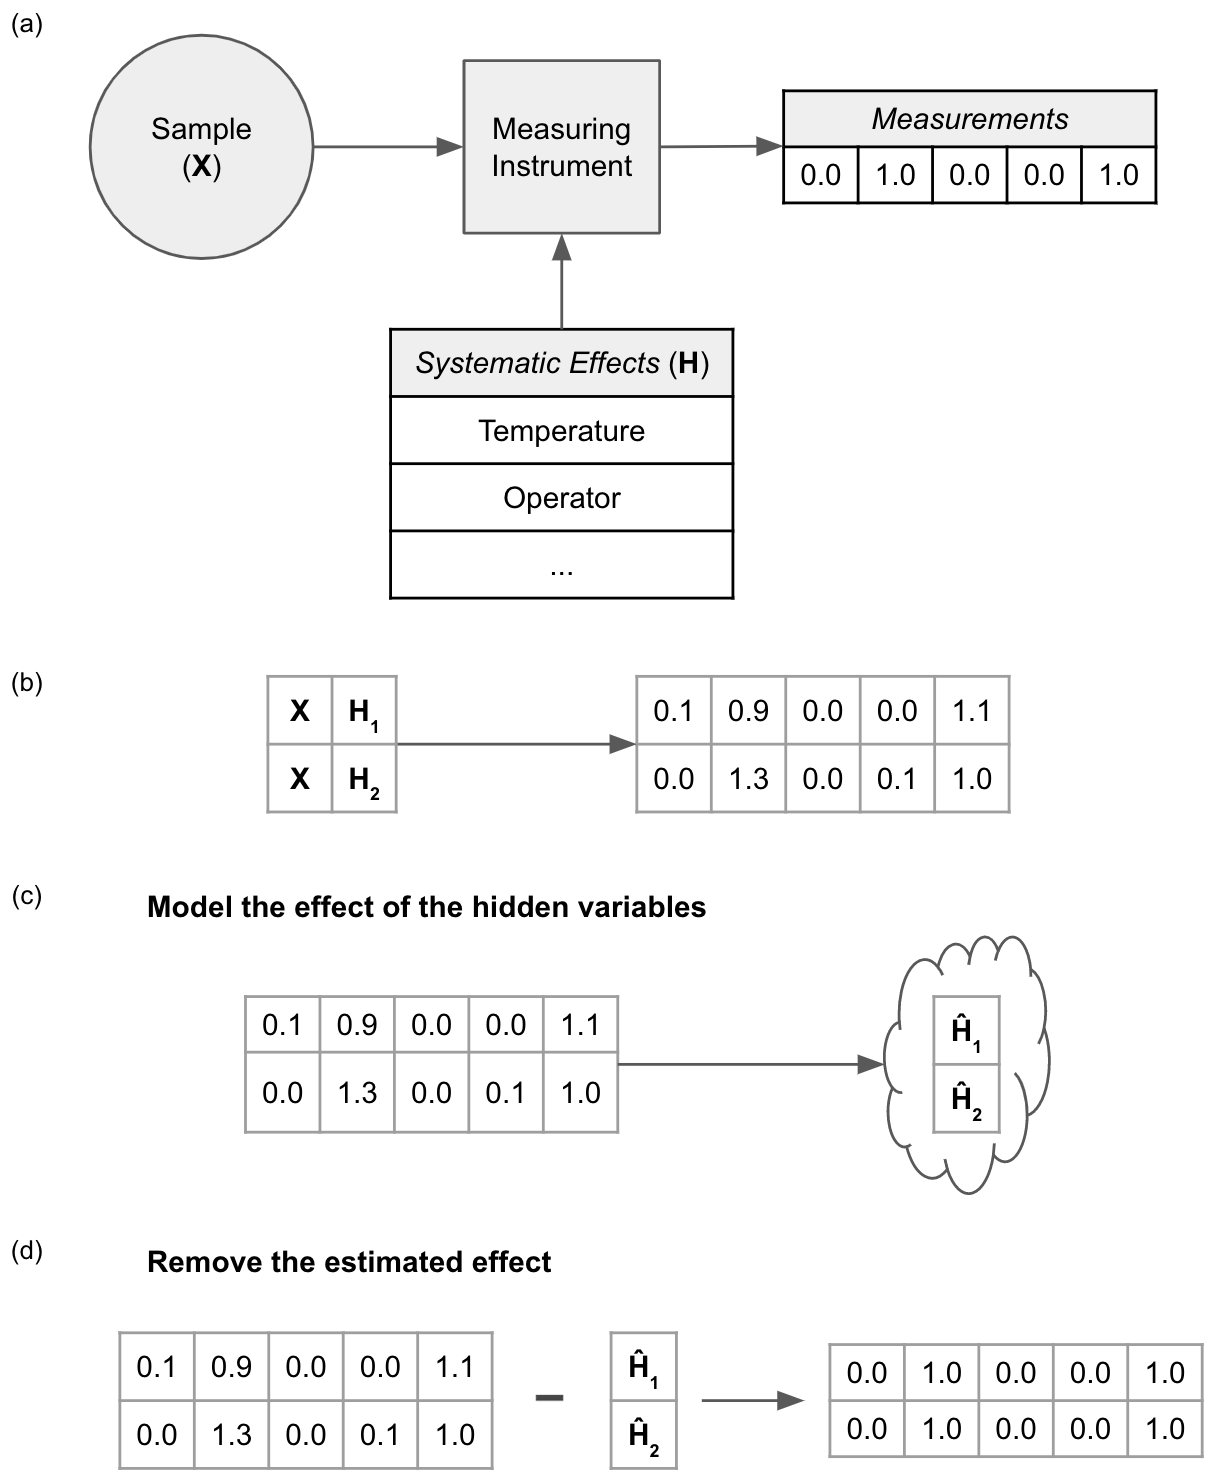
\includegraphics[width=4.5in]{figures/rough/adjuster_workflow}
	\caption{\textbf{Batch adjustment justification and steps} (a) When measurements are collected from a sample ($X$), systematic effects ($H$) also affect the measurements. (b) If data from the same sample $X$ is measured under two different conditions, $H_1$ and $H_2$, we may obtain slightly different measurements. (c) In orer to normalize batches of data relative to one another, we first estimate the effect of the hidden variables based on differences in measurements between batches. (d) Second, we remove the estimated effects in order to normalize the batches relative to one another.}
	\label{fig:workflow}
\end{figure}

Many tools have been developed to account and adjust for batch effects in expression data.
However, most of these tools only adjust for linear batch effects without accounting for nonlinear interactions between variables.
Because of the large number of features in expression data and the nature of these features (i.e. transcripts and proteins that interact biologically), we anticipate that these nonlinear effects may still be present even after adjustment with popular tools.
A few notable examples \cite{shaham_removal_2017,shaham_batch_2018} use deep neural networks to correct for batch effects, but these are optimized for use in large, balanced, dual-batched datasets and are therefore unusable for many real-world examples.

\textbf{Hypothesis:}
Using an adversarial neural network can correct for batch effects more completely than previous tools do. % clarify here what "more completely" means

\section{Implementation}

\emph{\href{https://bmcbioinformatics.biomedcentral.com/submission-guidelines/preparing-your-manuscript/software-article}{Oxford Bioinformatics' guidelines} say that you should have an "Implementation" section instead of Materials and Methods.}

\subsection{Network Structure}

We used an adversarial autoencoder network to model and remove the batch effects.
This network was structured in two parts: an autoencoder to replicate the input (expression) data and a discriminator to detect remaining batch effects in the autoencoder.
By penalizing the autoencoder for the discriminator's success, the autoencoder subnetwork learned over training to output the expression data with all signs of batch effects removed.
The neural network was implemented in TensorFlow under Python 3.6.
All layers in the network were fully connected and all activation functions were ReLUs \cite{agarap_deep_2018} except the final activations in the autoencoder and the discriminator, which used the sigmoid for their final activations.
We also tried replacing the ReLU activations with SELUs \cite{klambauer_self-normalizing_2017} but saw little if any improvement and therefore returned to using ReLUs.

We toyed with the idea of using convolutional layers \cite{krizhevsky_imagenet_2012-1} in the network because of their incredible success in the realm of image recognition.
We thought at first that a 20,000-dimensional vector of expression values was quite similar to a 200x100 image and that similar techniques could be used for both, which was encouraging because convolutional filters are quite efficient for processing images.
However, we were unable to devise a representation or arrangement of gene expression data points in which convolutional filters would make sense.
Although one could easily wrap a gene expression vector into two dimensions and arrange the genes by location in the genome, each data point fundamentally represents a completely different gene product.
Contrast this with image data, where each pixel represents the same data type (i.e. relative light intensities of some wavelength); if each pixel value was shifted to the left by one pixel, the image would still represent the same idea.
However, if each expression value were to be shifted one position to the left, it would in essence be like mistaking each gene product for another unrelated gene product.
Therefore, passing convolutional filters over a gene expression array, 1D or 2D, would not make sense since the relationship between a pair of consecutive genes is not necessarily analogous to the relationship between another pair of consecutive genes.
Because we couldn't justify any arrangement where spatial relationships between genes were consistently meaningful, we chose to only use fully connected layers in Confounded rather than convolutional layers.
We welcome any future intellectual advances that may allow convolutional networks and other image processing techniques to be applied to expression data.

\begin{figure}
	\centering
	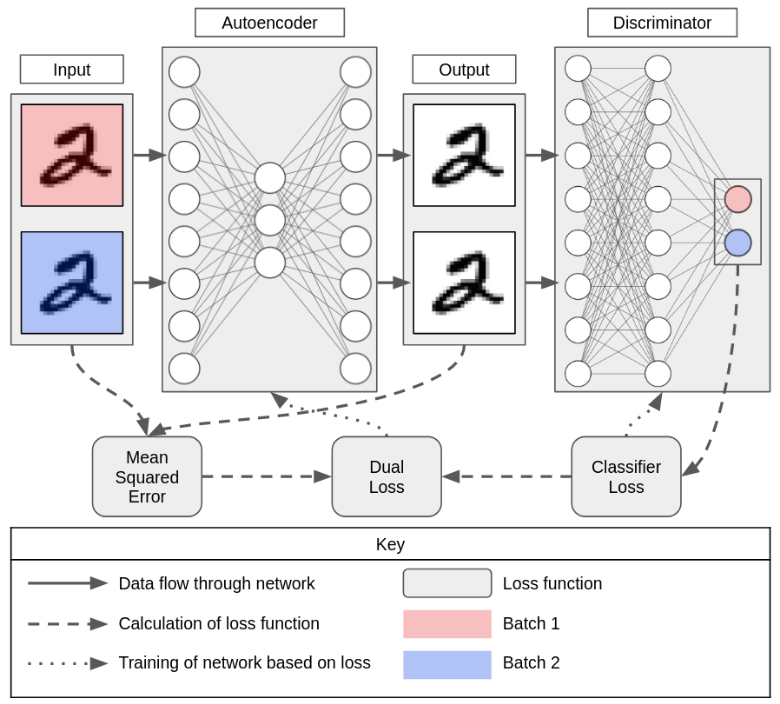
\includegraphics[width=4.5in]{figures/rough/network}
	\caption{\textbf{Network architecture} of Confounded. Data with batch effects (represented by different colors) are input into an autoencoder. The output of the autoencoder is classified by a discriminator network based on batch. The autoencoder is then penalized based on the success of the discriminator. Over time, the autoencoder learns to output a faithful representation of the data without signal due to batch.}
	\label{fig:network}
\end{figure}

\subsubsection{Autoencoder}

We initially implemented a basic fully connected autoencoder with two layers for encoding and two layers for decoding and with a smaller (about $\frac{1}{5}$ the size of the input) code layer.
In order to prevent overfitting while allowing sufficient complexity for identifying and removing higher-order batch effects we added dropout to all the layers with a probability of 50\%.
We tested this autoencoder with varying encoding and decoding layer sizes in order to determine the optimal balance of complexity and speed.
We also tested several variations on autoencoders; we implemented a variation on the U-Net \cite{ronneberger_u-net_2015} and plan to test the network with a variational autoencoder \cite{kingma_auto-encoding_2013}.
% TODO: implement and test the variational ae

\subsubsection{Discriminator}

The discriminator is given the output of the autoencoder and was trained to determine the original batch of that output.
It consists of a variable number of fully connected layers of size 500 and a one-hot encoded output for determining batch.
We noticed that the discriminator was overfitting on the data.
Since it memorized which sample belonged to which batch instead of learning batch-specific patterns, the only way for the autoencoder to fool the discriminator was to completely obfuscate the expression data, therefore also removing any relevant signal.
In order to combat this overfitting, we also added 50\%-probability dropout to each layer of the discriminator.
After adding dropout, the network appeared to no longer be overfitting.

\subsubsection{Loss functions}

Three loss functions were used to train the network.
First, the autoencoder was trained on mean squared error \ref{mse} ($MSE_A$) between the input and output layers.
Second, the discriminator was trained on mean squared error ($MSE_D$) between its output and a one-hot encoding of the samples' batch labels.
Finally, the autoencoder was also trained on a combination of the two previous losses,

\begin{equation}
	\label{dual_loss}
	Loss = MSE_A - \lambda{}(MSE_D)
\end{equation}

Where the $\lambda$ value represents a tradeoff parameter for tuning the network's tendency for more faithfully replicating the input or for more completely removing batch effects.

\subsubsection{Training}

In all cases, the network was trained using the Adam Optimizer \cite{kingma_adam_2014} with a training rate of either 0.001 or 0.0001.
We typically trained for 10,000 iterations on mini-batches of size 100.
This training typically took roughly 30 minutes to complete, including time spent to load the input and to save the output.

\begin{figure}
	\centering
	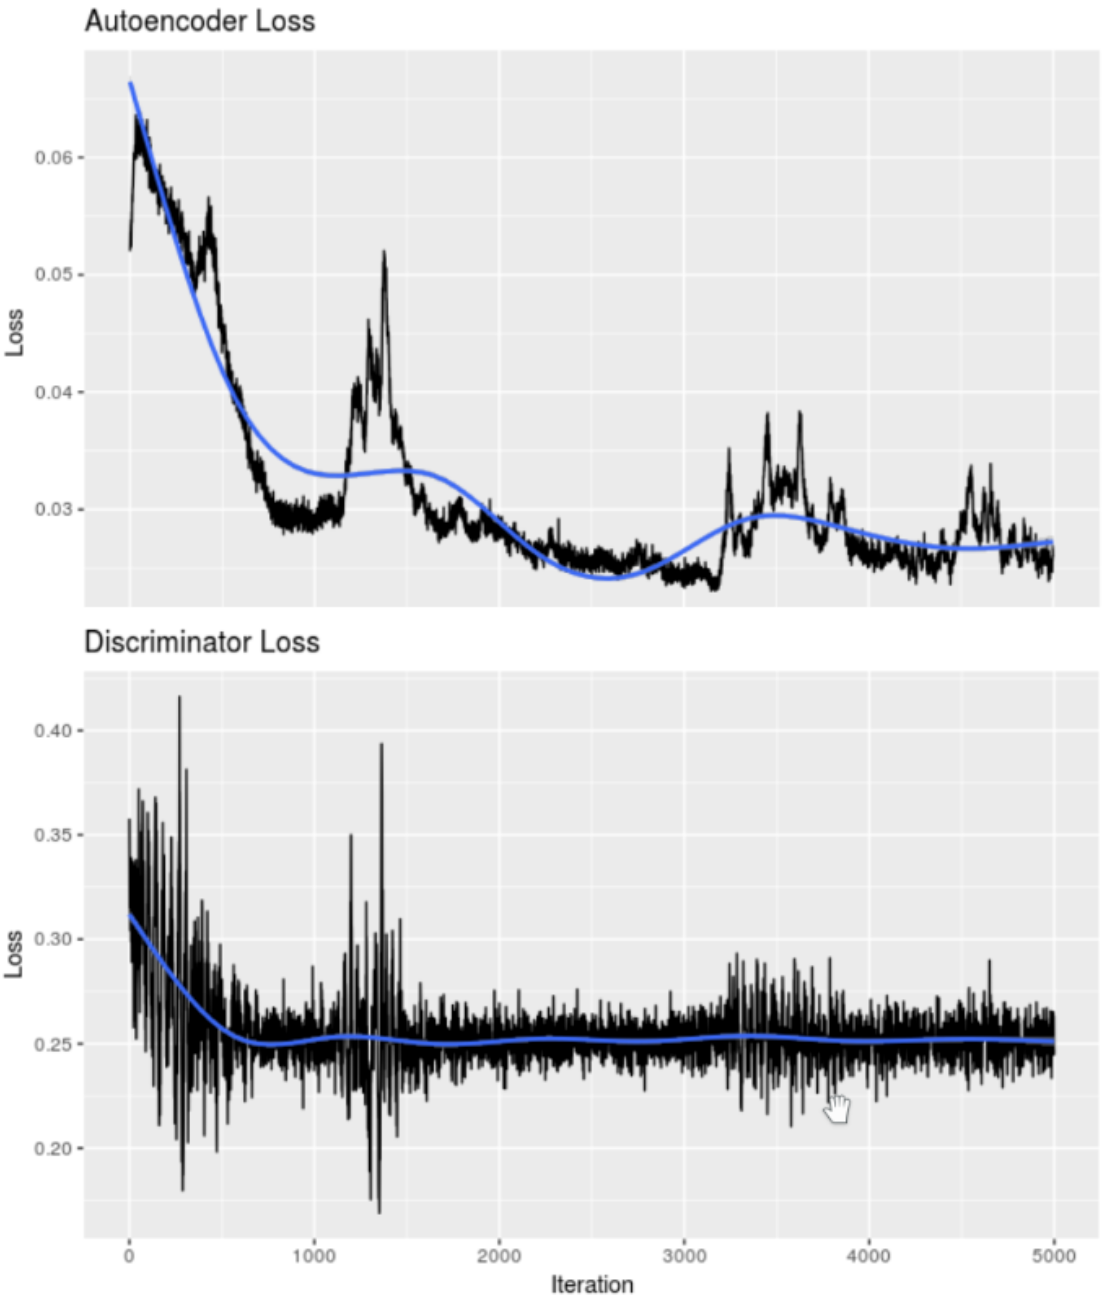
\includegraphics[width=4.5in]{figures/rough/training_loss}
	\caption{Autoencoder and discriminator loss over time for one run of Confounded. Over the course of training, the autoencoder more faithfully replicates the input data. The autoencoder also seems to introduce noise (see around iteration 3100) in response to the discriminator's slight improvements.}
	\label{fig:training_loss}
\end{figure}

\subsection{Datasets}

In order to test both theoretical and practical differences between Confounded and previous methods, we compared them for a variety of different datasets.
Working with each new dataset enlightened us of a new edge case that hadn't yet been addressed in our code.
By applying to our methods to each of the following datasets, our code became much more robust than if we had only developed and tested on one or two toy datasets.

\subsubsection{Data Format}

Confounded takes input data in the tidy data format \cite{wickham_tidy_2014-1}, namely:

\begin{itemize}
	\item Each row represents a different sample.
	\item Each column represents a different variable (either a clinical variable or a gene's expression).
\end{itemize}

Confounded parses through files in this format to determine which columns are discrete (integer or string) and which are continuous (floating point).
Each continuous column is interpreted to be a gene expression column and is adjusted for by the network according to the batch column.
This is one limitation to our software.
In a future iteration, it would be more robust to allow the user to specify continuous columns that should not be interpreted as gene expression data (e.g. ages in years with decimal precision representing fractions of years).
However for the datasets we tested, this didn't prove to be a problem.

\subsubsection{MNIST}

The MNIST digits dataset \cite{lecun_mnist_nodate} is a database of images of handwritten digits that are size-normalized and centered.
It contains 60,000 training images and 10,000 test images.
In order to use this dataset, we flattened each 28 by 28 image into a 1D vector of size 784 and put each in a CSV file along with the accompanying digit information.
We limited our dataset to only the 10,000 test images.

By using MNIST, we were able to visually assess how much true signal (in this case, the shape and digit of each handwritten digit image) is preserved after batch adjustment.
Although convolutional layers would typically be used when working with images such as the MNIST dataset, we chose to use only fully connected layers even for this image dataset.
In this way, we show that the autoencoder is still able to find and represent spatial relationships without explicitly defining spatial relationships in the model while testing the same network we use on expression data, where no spatial relationships are inherent.

\paragraph{Synthetic Batch Effects}

Because there is no batch information in the MNIST digits dataset, we had to simulate nonlinear batch effects.
To do so, we wrote a Python script that would take the MNIST data in, apply some nonlinear effect, and output the adjusted data.
We applied nonlinear effects by iteratively realizing vectors of normal values, multiplying and adding these vectors to the ``expression'' vectors, and applying nonlinearity to the adjusted vector.
We split the image data into two batches while keeping the batches balanced (5,000 images for each batch) and including the same number of each digit in each batch.
The same normal vectors were applied to each image in a batch.
Finally, random noise was added to each image in order to prevent images in a batch from being too similar to each other.

\subsubsection{Bladderbatch}

The bladderbatch dataset is a microarray transcriptome expression dataset from a study of patients with bladder cancer \cite{dyrskjot_gene_2004}.
It has been made available in an R package \cite{leek_bladderbatch_2017} and is used in the documentation of the sva R package to illustrate how to batch-adjust using ComBat \cite{leek_sva_2017}.
It contains expression values for 57 samples of patients with and without bladder cancer across 5 unbalanced batches.
Because it is such a small dataset in terms of typical deep learning datasets, we selected it as a way to test whether our network was overfitting.

\subsubsection{GSE37199}

The GSE37199 dataset contains microarray data from patients with advanced castration-resistant prostate cancer \cite{olmos_prognostic_2012}.
We accessed a version of this data from the Open Science Framework that was tidied as part of a curated compendium of human transcriptional biomarker data \cite{golightly_curated_2018}.
This represents a slightly larger dataset than bladderbatch with only two batches that are closer to being balanced.
Additionally, this dataset has two levels of batches (``centre'' and ``plate'').
We identified this as an item of potential interest: can Confounded adjust for multiple batch effects simultaneously?
However, we left this question for future research and chose instead to focus on the ``plate'' effect for the time being.

\subsubsection{TCGA Pan-cancer Data}

The Cancer Genome Atlas (TCGA) Pan-Cancer project produced expression data for thousands of tumors across many cancer types \cite{the_cancer_genome_atlas_research_network_cancer_2013}.
In a previous study, we used this dataset and attempted to remove the effect of tissue type from this dataset using ComBat \cite{dayton_classifying_2017-1}.
However, we found that a strong nonlinear signal could still be identified in the data after adjustment.
We used the same dataset that we tidied in this study to see if we could remove this nonlinear batch signal more completely.
This dataset has RNA-Seq expression values for 9,365 samples across 25 distinct cancer types.
We used this dataset as a way to test whether Confounded works on RNA-Seq data as well as to test whether we could remove batch effects that we know ComBat cannot.

\subsection{Other adjusters}

We compared our method to two other batch adjusters: a mean and scale adjuster and ComBat \cite{johnson_adjusting_2007}.
We implemented the mean and scale adjuster in the R programming language \cite{r_core_team_r_2014} and used the ComBat implementation from the sva package \cite{leek_sva_2017} with some modifications to allow it to work on columns without variance in the MNIST dataset.
We wanted to also compare with SVA \cite{leek_capturing_2007} and the Shaham lab's work \cite{shaham_removal_2017,shaham_batch_2018} but were unable to get these two methods to work.
With SVA, the documentation showed how to identify surrogate variables and use them in modeling, but we were unable to find examples of removing the effects that those surrogate variables represent.
We were unable to get the Shaham lab's methods running on our datasets, and we believe that this is due to some underlying assumptions in their code (see \ref{section:mmd} for more information).

\subsection{Statistics and Metrics}

In order to determine how well Confounded removes batch effects as compared to other batch correction software, we calculated several metrics.
First, we calculated mean squared error to see how different the output is from the input.
Second, we calculated sample maximum mean discrepancy to see how differently distributed the batches are from each other.
Third, we determined classification accuracy for several machine learning classifiers unrelated to deep neural networks based on batch in order to determine whether batch can still be identified post-adjustement.
Finally, we determined the same classification accuracies but based on ``true class'' labels to determine how well important signal is maintained after adjustment.

\subsubsection{Mean squared error}

Mean squared error (MSE) is a measure of how much two vectors or matrices deviate from one another.
It is commonly used as a loss value in autoencoders to make the network minimize the difference between the input and output values.
We used MSE as a constraint on the autoencoder in Confounded and wanted to see how well other batch correction software maintain patterns in the input data as measured by MSE.

We calculate MSE by the following:

\begin{equation}
	\label{mse}
	MSE = \frac{1}{n}\sum_{i=1}^n{(\hat{x}_i - x_i)^2}
\end{equation}

Where $x$ represents the values in the autoencoder's input and $\hat{x}$ represents the approximated values in the output.
If $x = \hat{x}$, MSE will be 0.

\subsubsection{Maximum mean discrepancy} \label{section:mmd}

A recent paper also used neural networks to remove batch effects \cite{shaham_removal_2017}.
Instead of constraining the autoencoder to remove batch effects based on a discriminator, these researchers trained their network to minimize maximum mean discrepancy (MMD) between batches in an embedded layer of their network.
We wanted to compare our network against this network, so we calculated MMD for each adjuster.
Unfortunately, we were unable to get their network to work on our datasets for comparison due to some assumptions in their code (there must only be two batches, the two batches must be perfectly balanced, and the dataset must be fairly large).
However, we still calculated this metric to determine whether batches looked like they came from the same distribution after adjustement.

We calculated MMD using the following formula:

\begin{equation}
	\label{mmd}
	MMD(x, y) = \frac{1}{n^2}\sum_{i=1}^n{\sum_{j=1}^n{k(x_i, x_j)}} - \frac{2}{nm}\sum_{i=1}^n{\sum_{j=1}^m{k(x_i, y_j)}} + \frac{1}{m^2}\sum_{i=1}^m{\sum_{j=1}^m{k(y_i, y_j)}}
\end{equation}

Where $k(x, y)$ is the Gaussian kernel between $x$ and $y$ as implemented in \texttt{sklearn.metrics.pairwise.rbf\_kernel}, and where $x$ represents the data from one batch and $y$ represents the data from another batch.
In cases where there were more than two batches (e.g. $x$, $y$, and $z$), we averaged the pairwise MMD values to calculate an overall MMD:

\begin{equation}
	\label{mmd-mean}
	MMD_{total}(x, y, z) = \frac{1}{3}[MMD(x, y) + MMD(x, z) + MMD(y, z)]
\end{equation}
% TODO: make this formula ^ apply to more than 3 batches

\subsubsection{Classification accuracy}

We used four classifiers from the scikit-learn Python library in order to classify on batch and true class before and after adjustment: Naive Bayes, Random Forests, k-Nearest Neighbors, and SVM with a radial basis kernel.
Our true classes were as follows:

\begin{itemize}
	\item MNIST: digit
	\item bladderbatch: presence of cancer
	\item GSE37199: stage of cancer
	\item TCGA: presence of a TP53 mutation
\end{itemize}

We calculated the average of classification accuracies for four-fold cross-validation repeated 10 times.
We interpret lower accuracy for batch classification as meaning that the batch is removed more effectively.
We also interpret higher true class classification as meaning that the important signal is not lost during the process of adjustment.
Therefore, given output data from the ideal batch adjuster, batch classification would be no better than random for any classification algorithm, and true class accuracy would be no lower than accuracy for the unadjusted data.
We report these values in section \ref{results}.
% TODO: ^ This

\section{Results} \label{results}

% TODO: put all the figures in here

\subsection{Effects are still detectable after ComBat and scale adjusting}

\subsection{Effects not removed by other adjusters are removed by Confounded}

\subsection{Important signal is not removed by Confounded}

\begin{figure}
	\centering
	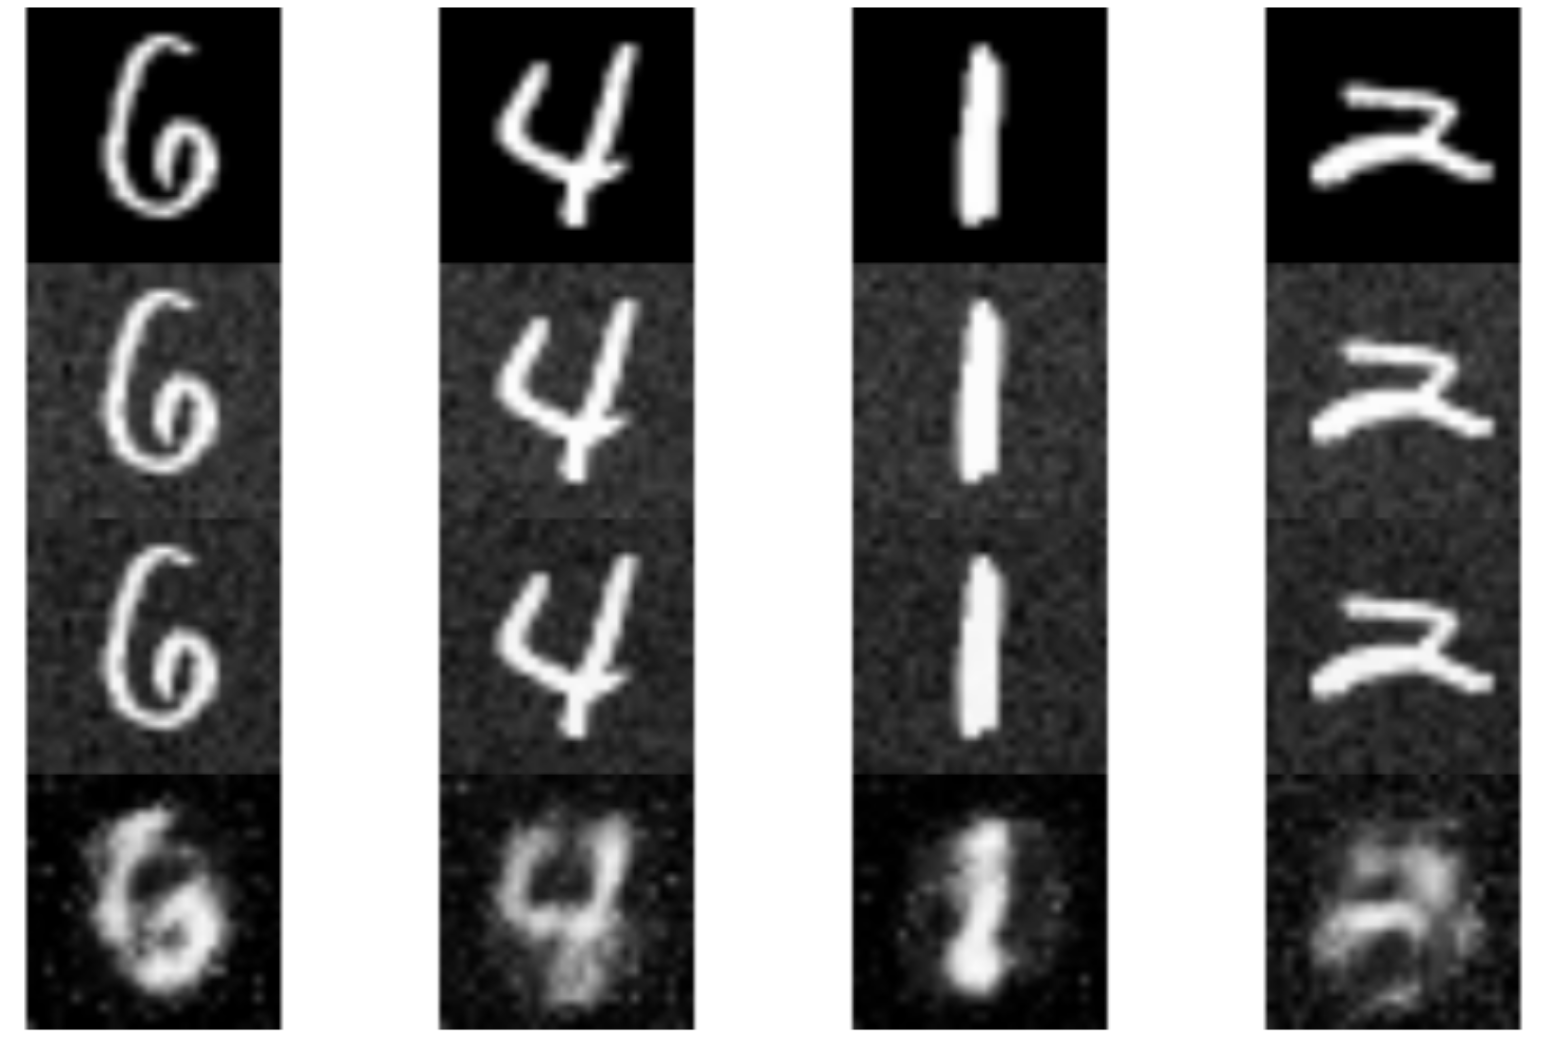
\includegraphics[width=4.5in]{figures/rough/mnist}
	\caption{\textbf{MNIST handwritten digits} (a) before any adjustment, (b), with artificial noise added, (c) adjusted for noise by ComBat, and (d) adjusted for noise by Confounded. Although Confounded seems to remove more noise from the background and make it look more like the original background, it struggles in some cases to accurately replicate the input data.}
	\label{fig:mnist}
\end{figure}\begin{figure}
	\centering
	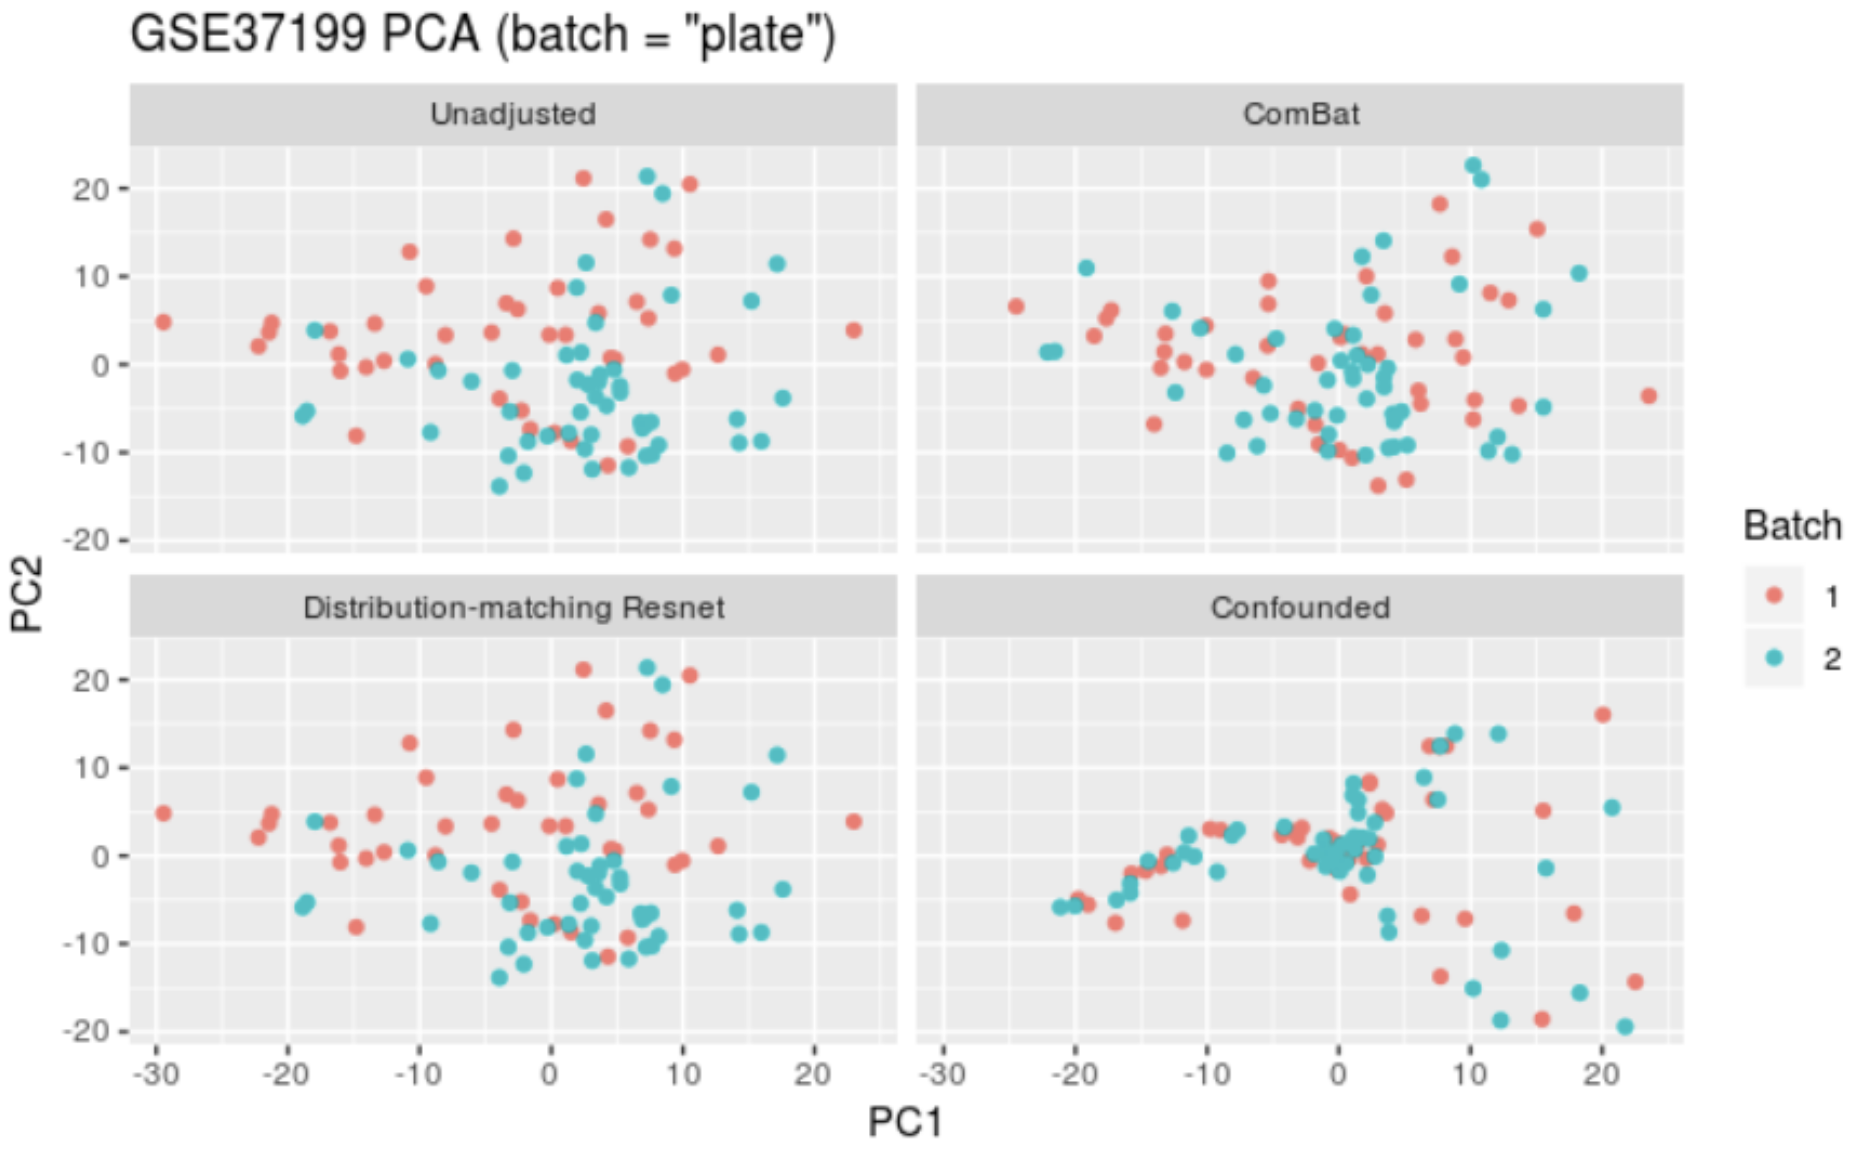
\includegraphics[width=4.5in]{figures/rough/pca}
	\caption{\textbf{Principal components analysis} (PCA) of the GSE37199 dataset before and after batch adjustment with various adjusters.}
	\label{fig:pca}
\end{figure}
\begin{figure}
	\centering
	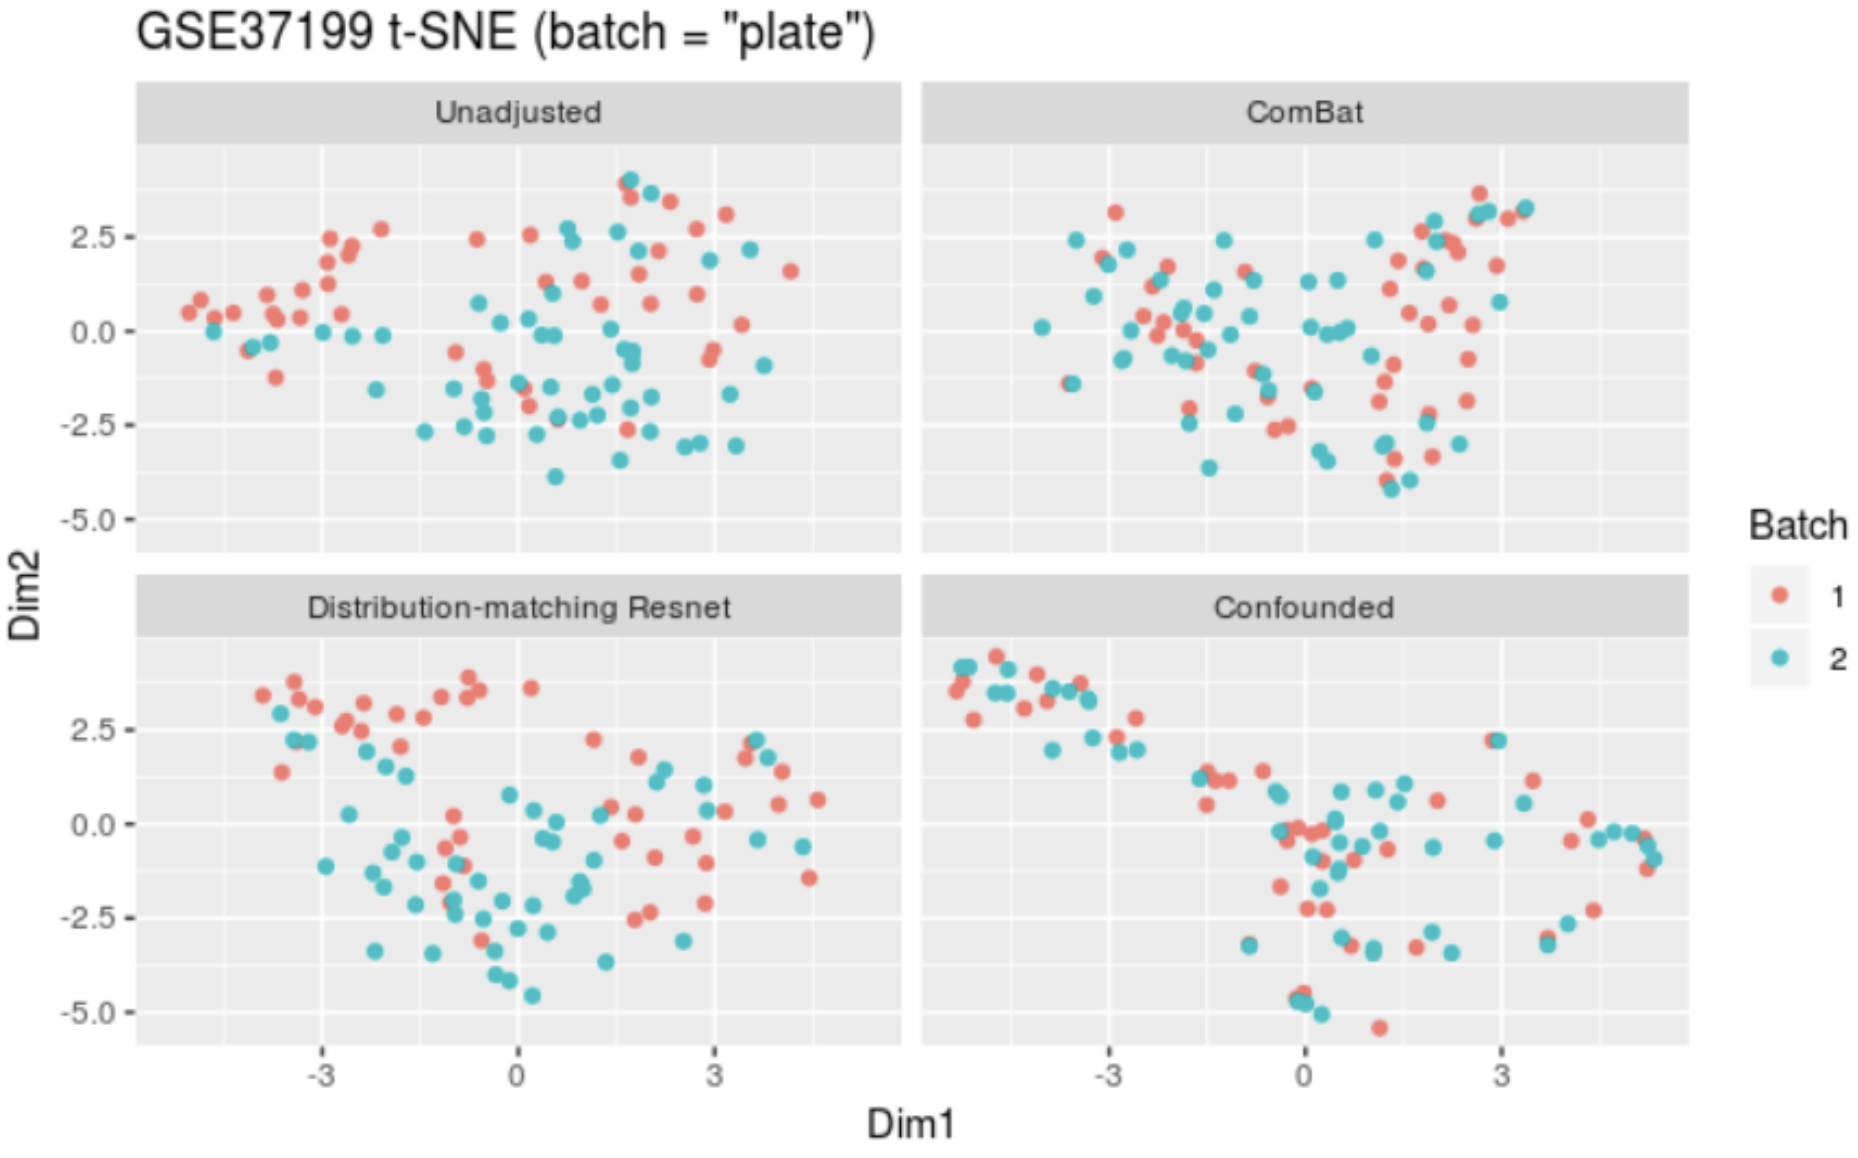
\includegraphics[width=4.5in]{figures/rough/tsne}
	\caption{\textbf{T-distributed Stochastic Neighbor Embedding} (t-SNE) plot for the GSE37199 dataset before and after adjustment with several algorithms.}
	\label{fig:tsne}
\end{figure}
\begin{figure}
	\centering
	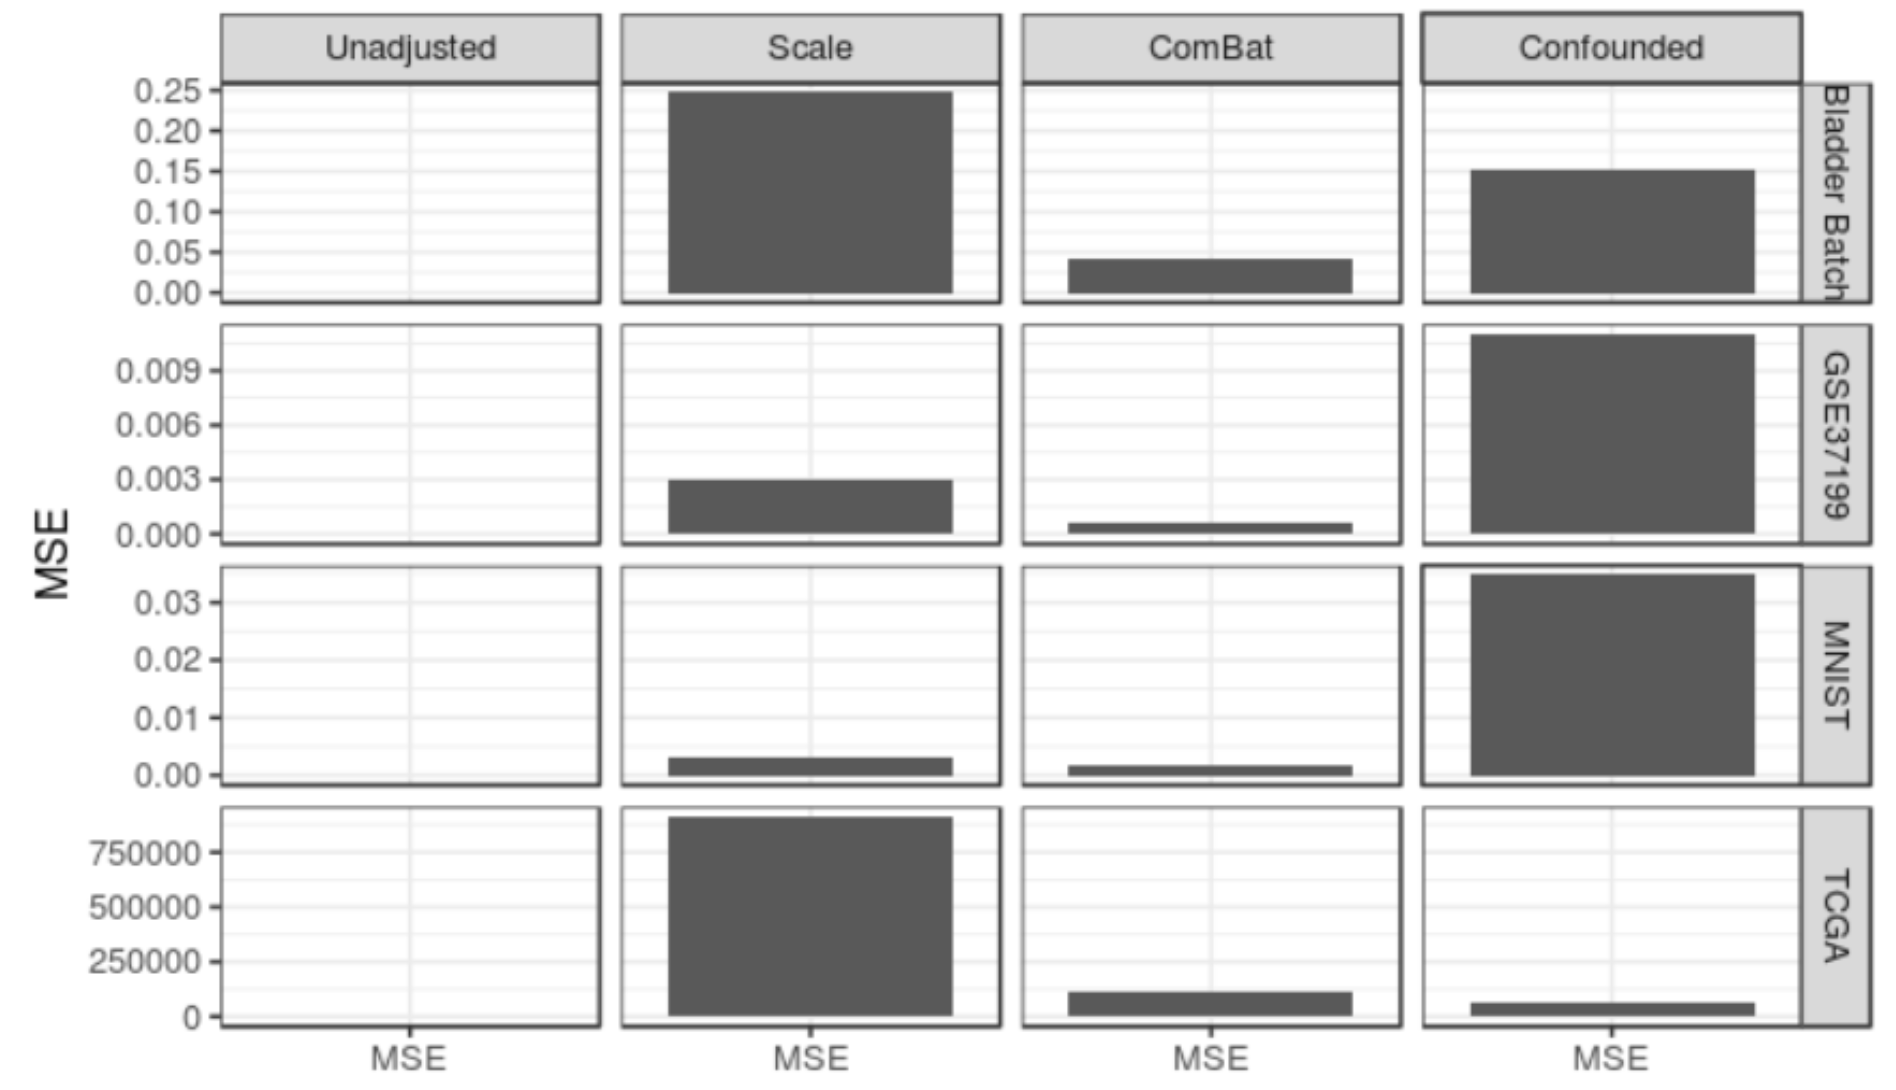
\includegraphics[width=4.5in]{figures/rough/mse}
	\caption{\textbf{Mean squared error} (MSE) between the data prior to and after adjustment with various algorithms.}
	\label{fig:mse}
\end{figure}
\begin{figure}
	\centering
	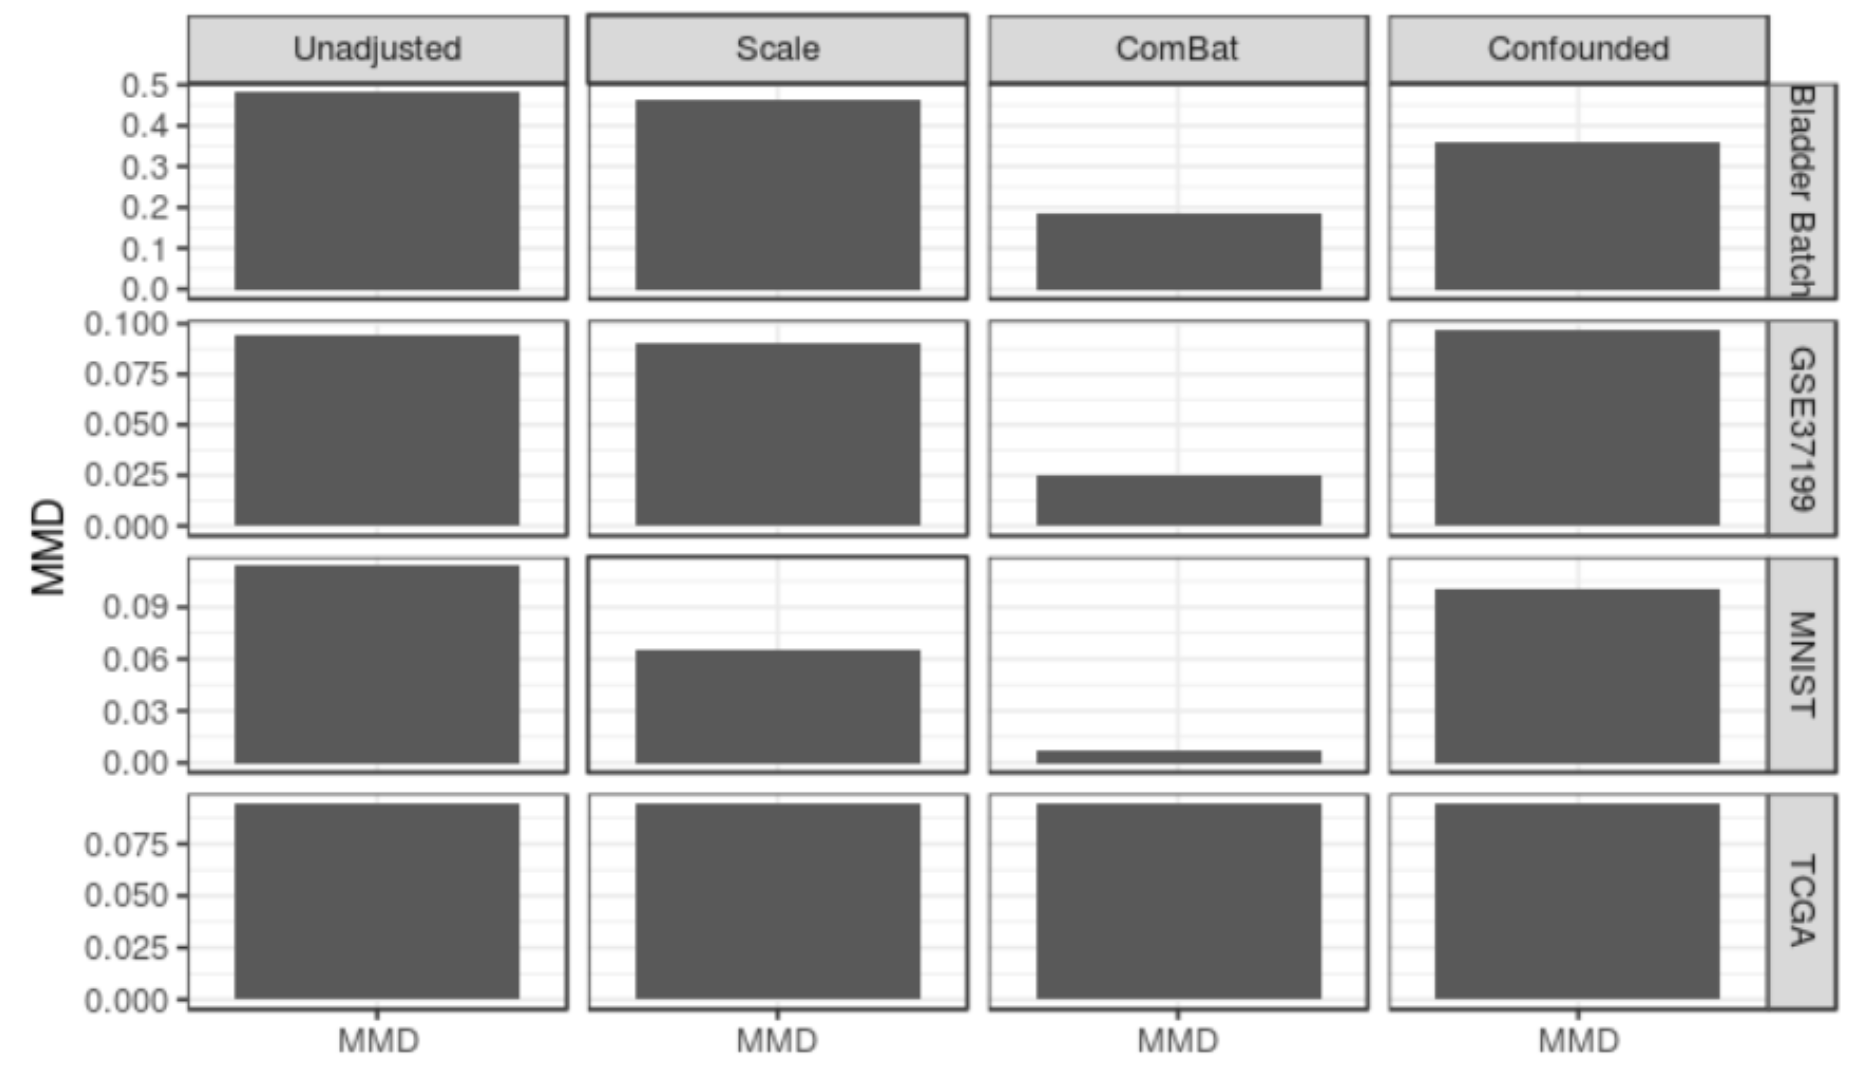
\includegraphics[width=4.5in]{figures/rough/mmd}
	\caption{\textbf{Maximum mean discrepancy} (MMD) between different batches. In cases with more than two batches, MMD is computed pairwise between each batch and averaged.}
	\label{fig:mmd}
\end{figure}
\begin{figure}
	\centering
	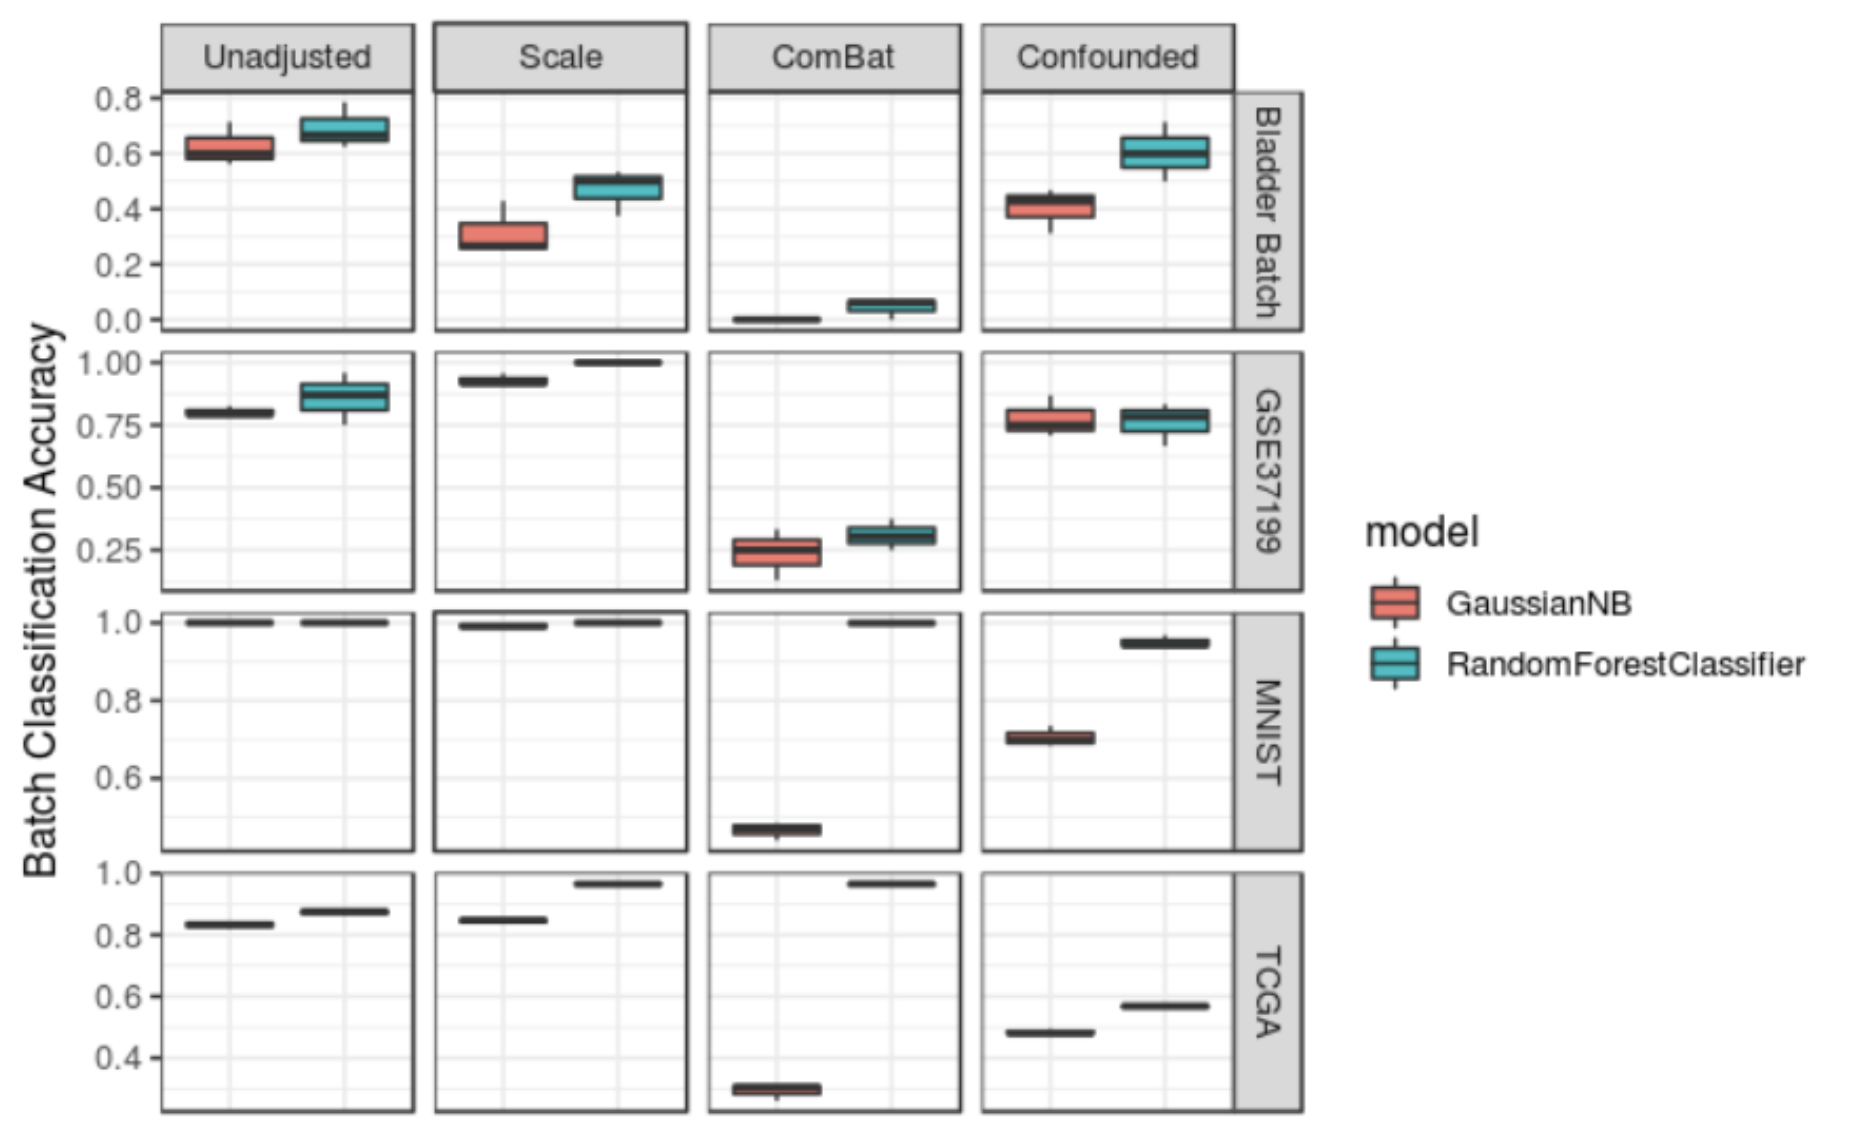
\includegraphics[width=4.5in]{figures/rough/batch_accuracy}
	\caption{\textbf{Batch classification accuracy} Accuracies for batch classification for 4-fold cross validation repeated 10 times for several classifiers.}
	\label{fig:batch}
\end{figure}
\begin{table}
	\centering
	\csvautotabular{figures/rough/batch.csv}
	\caption{Batch classification accuracy}
	\label{tab:batch}
\end{table}
\begin{figure}
	\centering
	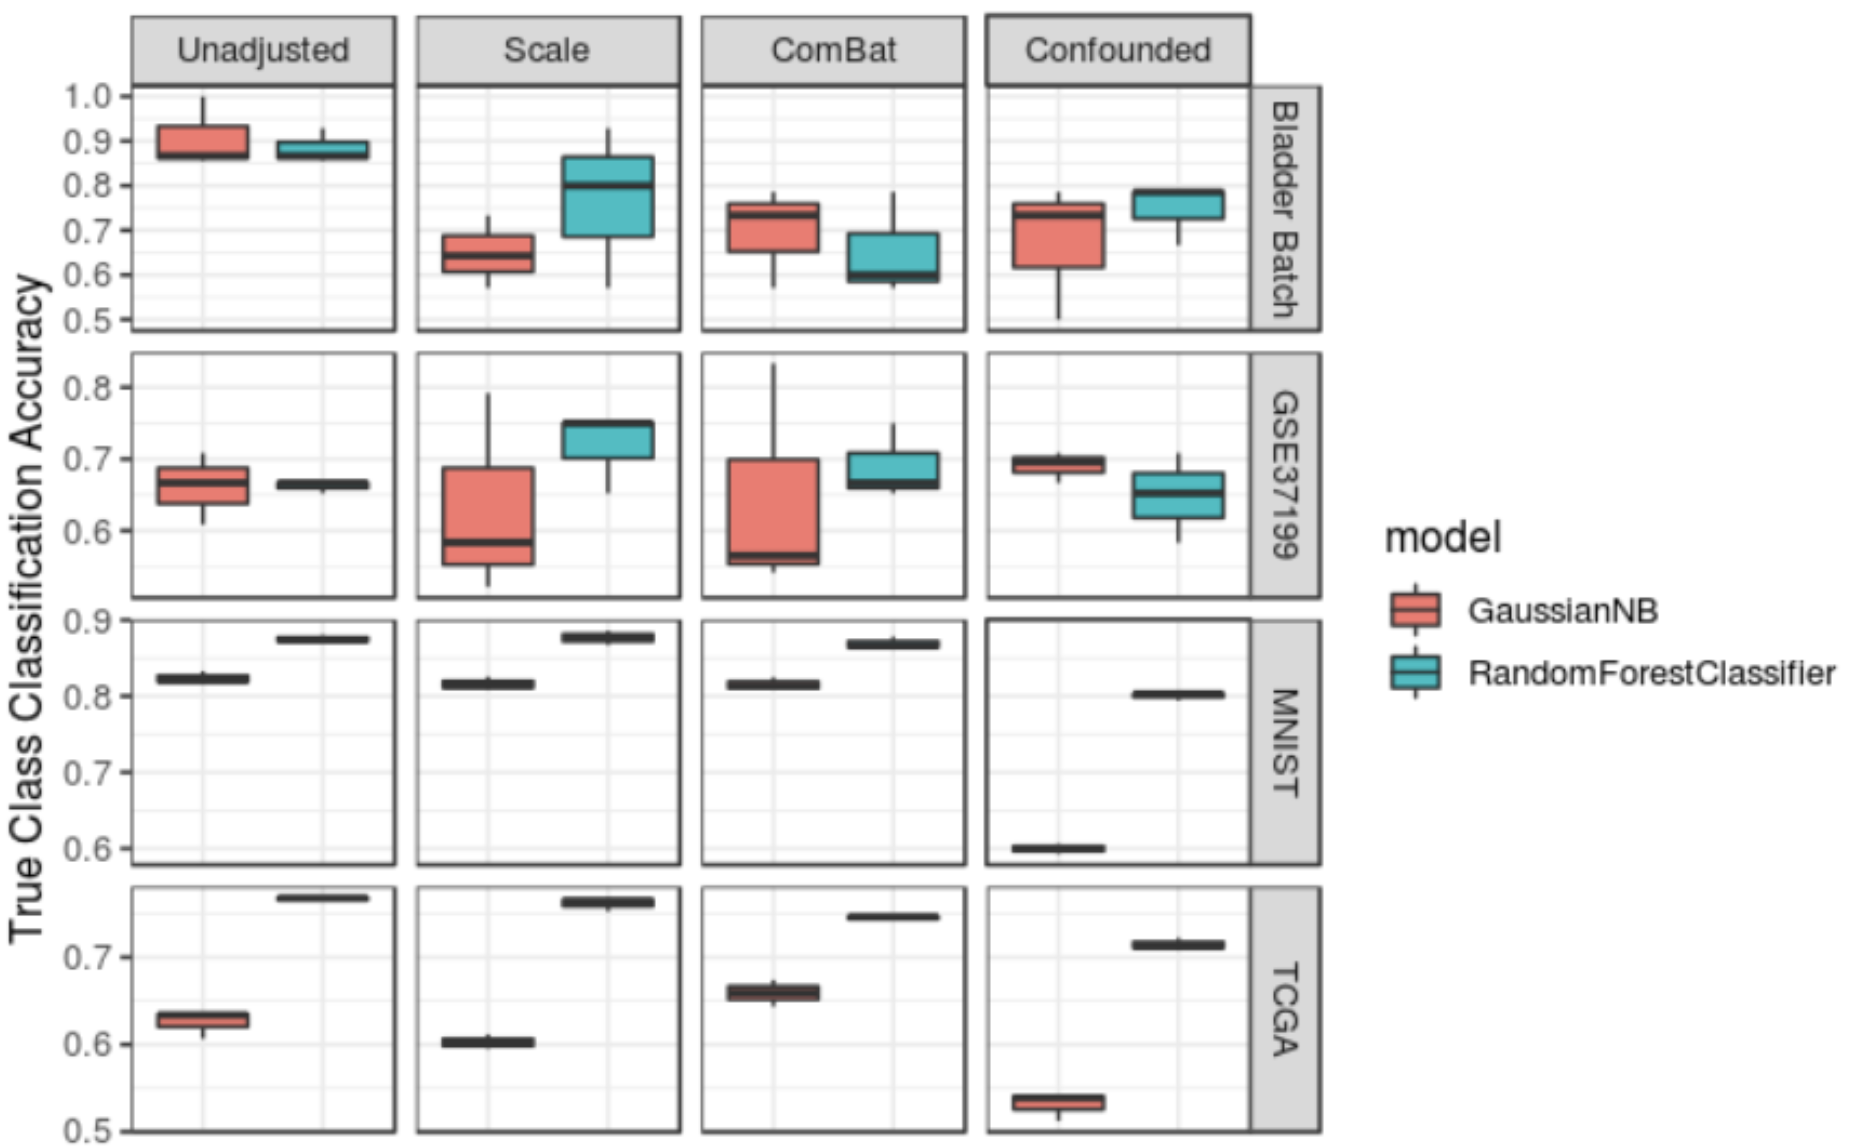
\includegraphics[width=4.5in]{figures/rough/true_class_accuracy}
	\caption{\textbf{True class classification accuracy} for several datasets and adjusters.}
	\label{fig:true_class}
\end{figure}
\begin{table}
	\centering
	\csvautotabular{figures/rough/true_class.csv}
	\caption{True class classification accuracies}
	\label{tab:true_class}
\end{table}

\section{Discussion}

\section{Conclusions}

\bibliography{references}

\end{document}
